\documentclass{llncs}


\usepackage{subcaption}
\usepackage{changepage}
\usepackage{authblk}
\usepackage{float} %% สำหรับวางรูปภาพ
\usepackage{graphicx}
\usepackage{amsmath}

\title{ Hanuman-KMUTT: Team Description Paper }
%\medskip
\author{ Kongkiet Rothomphiwat \and Chattarin Rodpon \and Nasrun Hayeeyama \and Thirawat Chuthong \and Wisanu Jutharee \and Thavida Maneewarn }

%\affil{\medskip King Mongkut’s University of Technology Thonburi
%	Institute of Field Robotics (FIBO)
%	126 Pracha u-tid Rd., Bangmod, Thungkru, Bangkok 10140, Thailand 
%	praew@fibo.kmutt.ac.th}
\institute{ King Mongkut's University of Technology Thonburi \\ Institute of Field Robotics (FIBO) \email{praew@fibo.kmutt.ac.th}}

\date{December 2018}

\begin{document}
	\maketitle
	
	
	\begin{abstract}
		This paper describes the design and development of the kid-sized humanoid robots of the Hanuman-KMUTT team for RoboCup 2019 Humanoid League (Sydney, Australia). This paper will include system overview, vision module and next goal for development.
	\end{abstract}
	
	\section{Introduction}
\paragraph{}
Institute of Field Robotics(FIBO) at King Mongkut's University of Technology Thonburi (KMUTT) has developed the humanoid robots to participate in RoboCup humanoid kid-sized league since 2005 under the name 'Team KMUTT' and later on 'Pheonix'. The successor, 'Hanuman-FC', won the Thailand Humanoid Soccer Robot Championship 2012 and participated in World-RoboCup 2013 (Eindhoven, Netherlands) under the name 'Hanuman-KMUTT'. In World-RoboCup 2013, our team passed into the quarter-final round. At the end of 2013, Our team won the Thailand Humanoid Soccer Robot Championship 2013. And then we joined the World-RoboCup 2014 (João Pessoa, Brazil) and passed into round robin 2. Because of limited funding and Thailand has no longer host the local competition in the country, our humanoid team development has been suspended. Last year, Robocup Asia-Pacific 2017 were host in Thailand, We participated after 3 years break with new undergraduate members. This year ...
\paragraph{}
In this paper, we will describe the recent development of our kid-sized humanoid robots. Section 2 gives an overview of the system design in our robots which consists of two strikers and one goalie. In section 3, the vision based navigation system of the robot will be explained. Section 4 discusses the game control and decision-making system. The last section concludes the paper.
	\section{System overview}
Our robots hardware does not change much since Robocup Asia-Pacific in 2017 which consist of 5 robots comprised of 2 sizes; 3 with 57 cm tall, and 2 with 47 cm as shown in Fig \ref{fig:humanoid}. Each robot have mechanical hardware, sensors, computing hardware and 20 Dynamixel servo-motor. The structure of all robots is made of aluminum alloy sheet metal(details are provided in the robot specification sheet).
\begin{figure}[H]
	\centering
	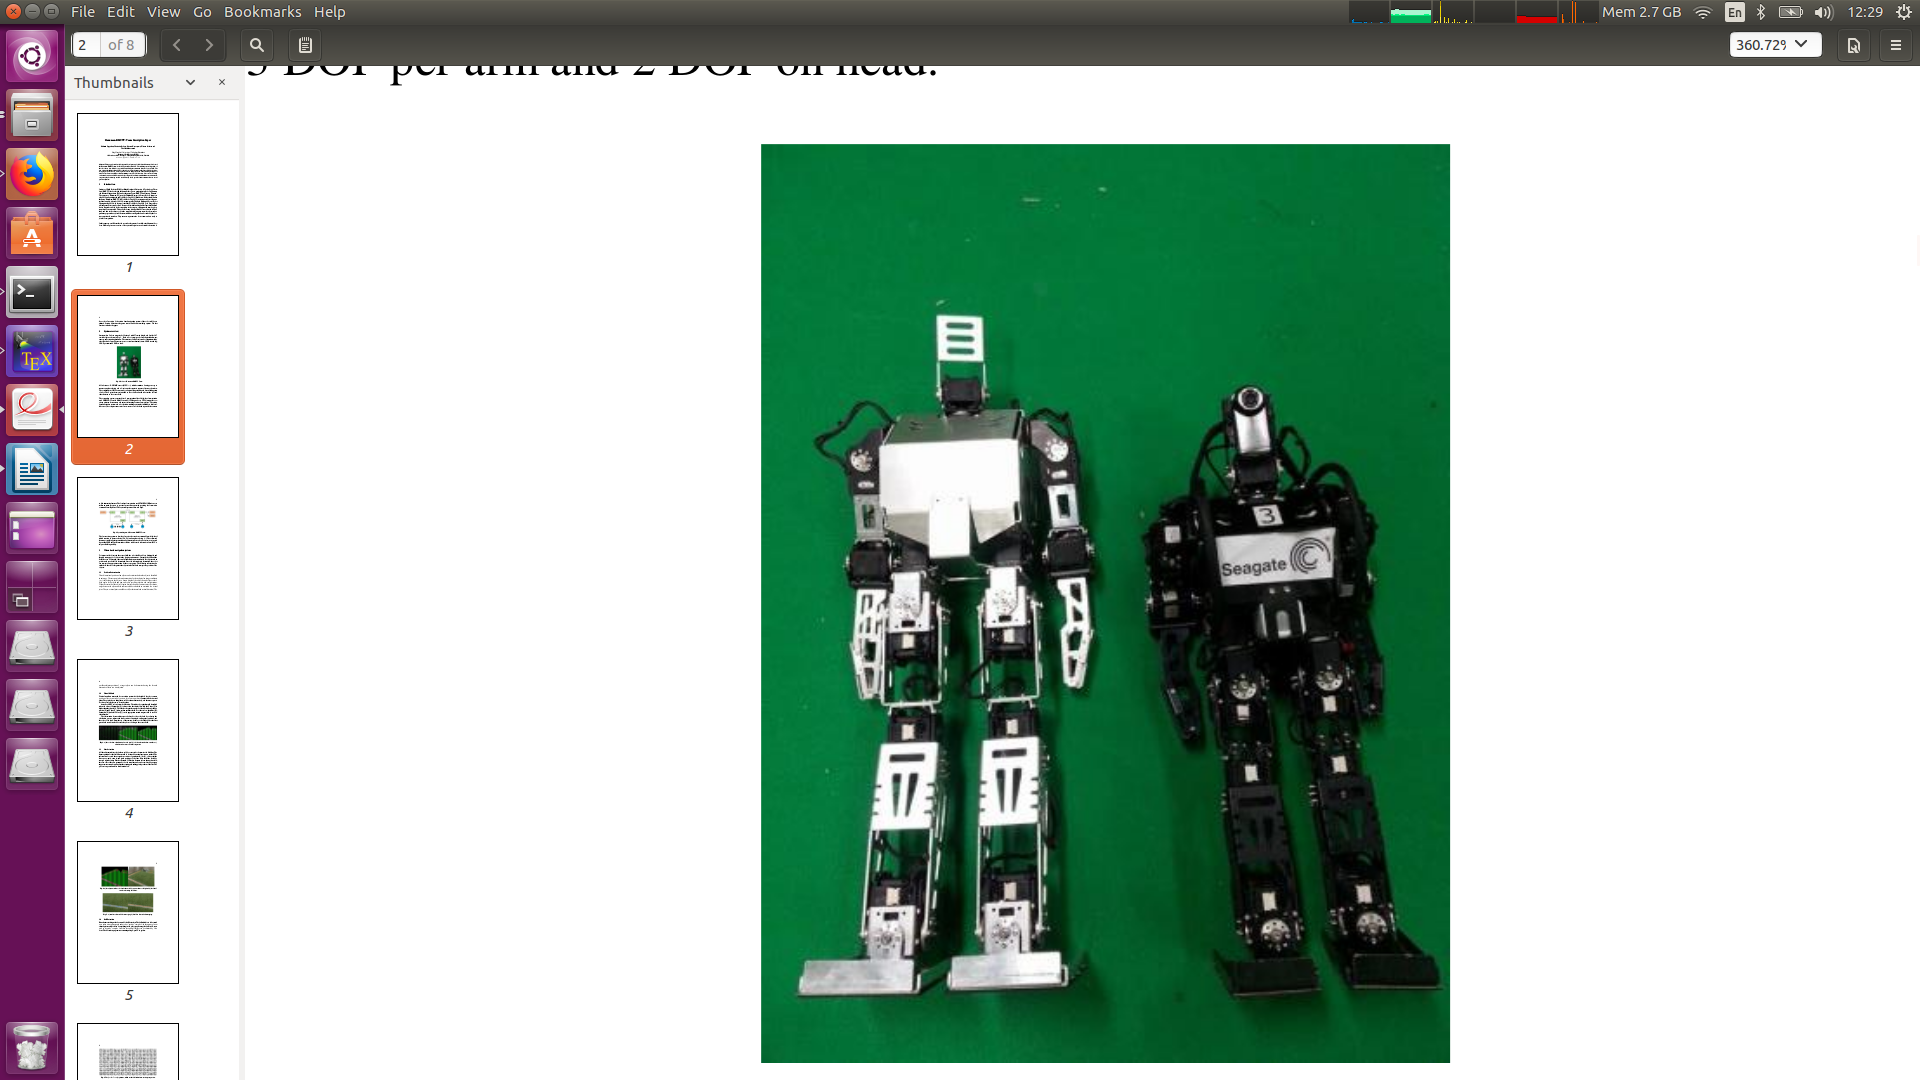
\includegraphics[width=\textwidth,trim={15cm 0cm 5cm 5cm},clip]{image/humanoid.png}
	\caption{Robots of Hanuman-KMUTT Team}
	\label{fig:humanoid}
\end{figure}
All robots use 6 DOF IMU sensor (MPU- 6500 ) which contains a 3-axis gyroscope and a 3-axis accelerometer. The combination of IMU sensor used to adapt walking stability and detect falling state of robot. The Logitech camera installed. The computing system consist of 2 separate systems; high-level and low-level as we described in \cite{TDP:Nakarin}. High-level computation used DROID-C1+ with ARM Cortex-A5 (1.5Ghz quad core CPUs) for computing image processing, decision making and navigation. Low-level computation used STM32F411RE micro-controller for operating locomotion system.
\begin{figure}[H]
	\centering
	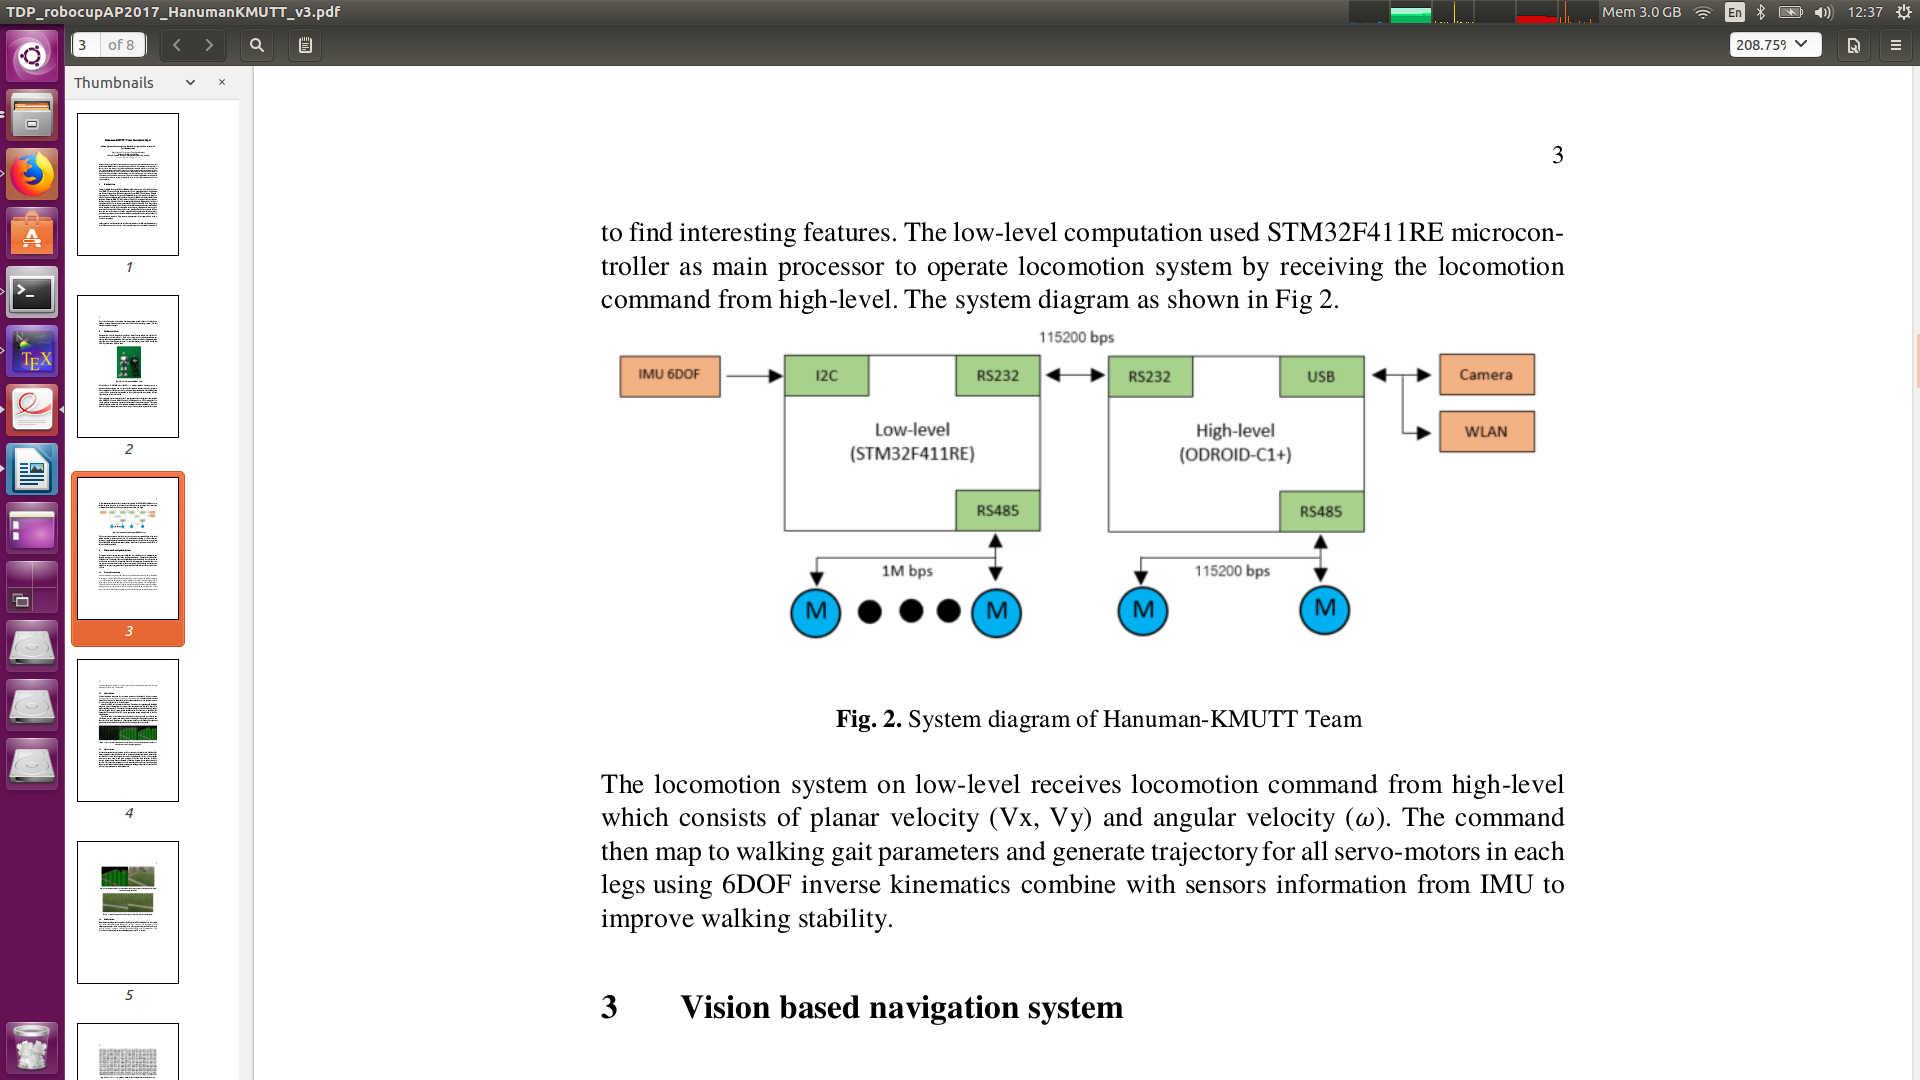
\includegraphics[width=\textwidth,trim={20cm 15cm 10cm 12.5cm},clip]{image/sysDiagram.png}
	\caption{System diagram of the computing system in the Hanuman-KMUTT Team}
	\label{fig:sysDiagram}
\end{figure}
	\section{Vision based navigation system}
\paragraph{}
To interact with objects in the soccer field, the robot shall be able to distinguish and identify many types of objects in the playing environment. Currently the ball and field lines can be detected, other useful information associated with the objects such as position and speed shall be determined. Once the information is determined, the robot can compute an appropriate action for the soccer game. Following subsections describe how the robot recognizes objects in the field and compute the position of objects. Moreover, information outside the soccer field can be useful since there is no landmark for robot to recognize which side is friendly territory. We found a method which have a potential to detect some objects outside the field.

	\subsection{Position Determination}
	\label{threeToTwo}
	\paragraph{}
	Three dimensional position of an object can be estimated when the object is identified in an image. The necessary information consists of a selected pixel on image coordinate (u, v) that belong to the object, forward kinematic from a robot base to a camera and camera's properties. Coordinate of interested pixels will be projected to a plane (floor) using perspective transform then three dimensional position which respect to robot base will be calculated using forward kinematic.
	
	\subsection{Color Segmentation}
	\label{colorSeg}
	\paragraph{}
	Each pixels in an image will be classified into eight colors (green, black, orange, blue, yellow, magenta, cyan and white) base on their pixel value. Then, apply watershed segmentation to get a better result on color segmentation.
	\paragraph{}
	We used HSV color system for classify a color of each pixels.The white color pixels would classified when the value of Saturation (S) is lower than the threshold, while the Value (V) is higher than the threshold. Black color pixels can also be classified when both Saturation (S) and Value (V) is lower than each threshold. For other colors, their Hue (H), Saturation (S) (and also Value (V)) on the appropriate certain ranges could be used for classification.
	
	\subsection{Field Boundary Detection}
	\paragraph{}
	An information about field boundary is importance for our soccer robot. This information can be used later on other image processing algorithm. We detect a field boundary by scanning an image from top to bottom and find a first green pixel for each columns of an image. Convex hull from those points we get by scanning an image will be our field boundary. 
	
	\subsection{Ball Detection}
	\paragraph{}
	From the competition in Robocup asia pacific 2017 [2] we have tried to used HAAR feature for ball detection. A lot of false positive detections have been occurred, so we have to remove out the un-related background by ignore every object outside a field boundary. The approach for ball detection has been slightly changed as followed.
	\begin{enumerate}
		\item As the ball contains white component mostly, the white color segmentation from \ref{colorSeg} has been used. Ramer–Douglas–Peucker algorithm [3] was used to classify how well the circle shape the object is. And then the region of the interests (ROI) of the detected objects would be used for consideration.
		
		\item The ROI(s) from previous step were checked with well-trained HAAR cascade classifier (using adaboost) [4][2].  Because we have limited the ROI(s), the scanning is faster than before. 
	\end{enumerate}
	
	\subsection{Line Detection}
	\paragraph{}
	Line information should bee useful for localization in future work. To detecting a line, we scan an image inside a field boundary from top to bottom every 8 image columns and find points where color is change from white to green. Three dimensional coordinate of those point can be obtained as we mention in \ref{threeToTwo}. Those points on a field line can be treat like a point cloud from laser scanner and be used by particle filter.
	
	
	
	\section{Game Control and Decision-making}

	\subsection{Game Controller}
	\paragraph{}
	To control the operation during the game, all robots continuously receive the message from the referee’s game controller. When the received message indicates the change of	the game state, the current operation is terminated. Then the robot loads the new operation which associated with that state.
	
	\subsection{Decision Making System}
	\paragraph{}
	The decision making system of all striker robots can be described by the finite state machine illustrated in figure below. The conditions for state changes of each state are determined based on the observation data from the vision system and internal sensor reading of the robot. In addition, the robot shares this information among the teammates
	by broadcasting mechanism via WLAN network. Therefore, the robot can cooperate to score the game as a team. The goalie decision can be described in a simpler state machine. The goalie is looking for the ball, if the ball heads toward the goalie on either direction (left/right). The goalie will fall in that direction in order to block the ball.
	\begin{figure}[H]
		\centering
		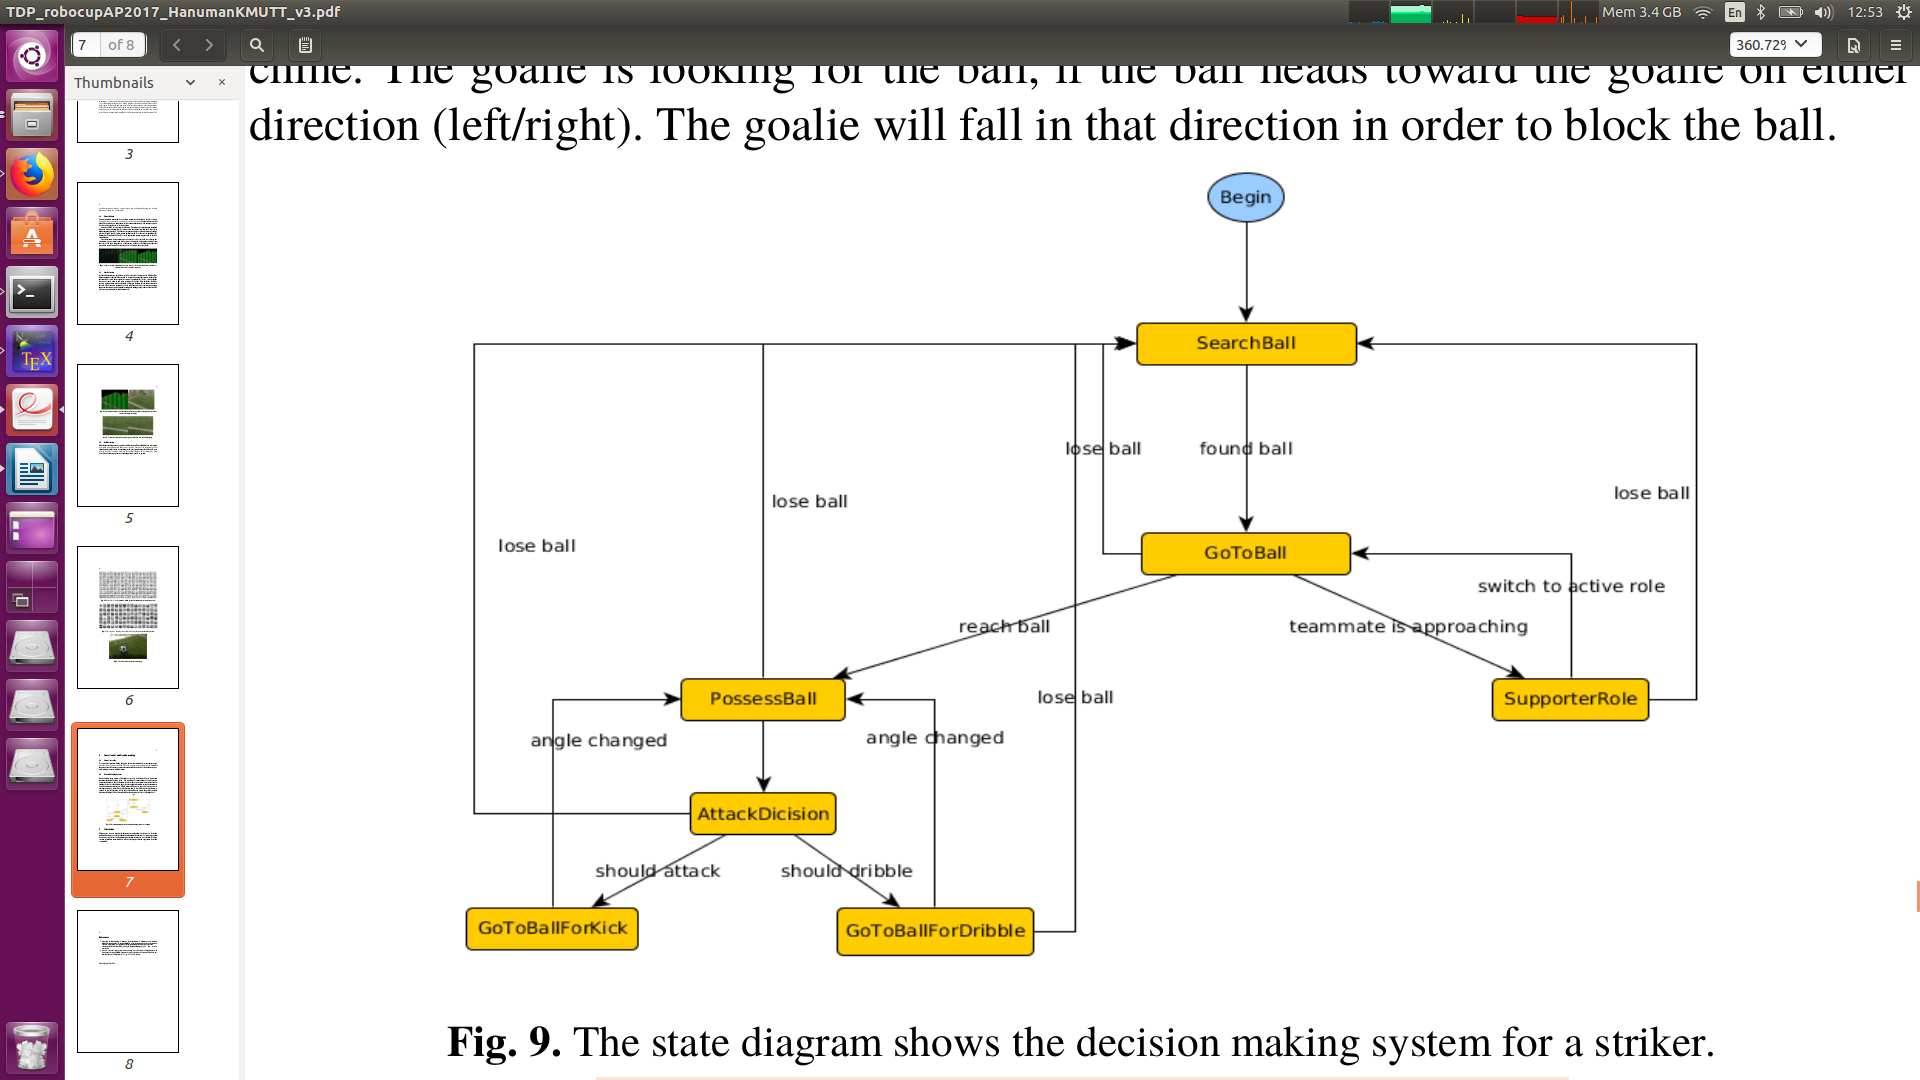
\includegraphics[width=\textwidth,trim={15cm 3cm 5cm 5.2cm},clip]{image/stateMachine.png}
		\caption{The state diagram shows the decision making system for a striker.}
		\label{fig:stateMachine}
	\end{figure}
	\section{Future Work}
	\subsection{Localization}
		Localization is important process in humanoid soccer. Robot cannot make decision correctly without knowing where it is. Hence, our goal of development for the next 6 months is to make localization system available for our robots. Object detection such as field boundary detection, lines detection and a new concept about landmark detection will be combined which will allow us to be closer to our goal of vision based localization.
		
		\paragraph{}
		Particle filter is one of interesting algorithm for localization in humanoid soccer robot since map of a field is known before hand. Our information from line detection will probably enough for this algorithm. A problem that we expect is symmetry of field which can cause robot to be confused about it heading direction. This problem will probably be handled by giving a robot an initial state or landmark detection if it's proven to be suitable for our problem.
	
	\bibliographystyle{splncs04}
	\bibliography{ieee} 
	
	
	
\end{document}